\chapter{Visualizing Output in ICE}
\label{sec:visOutput}
Currently, ICE features two plugins for visualizing and plotting
simulation output data:

\begin{itemize}
\itemsep1pt\parskip0pt\parsep0pt
\item
  \textbf{VisIt Tools} - An interactive 3D visualization tool for
  rendering meshes, scalar plots, contour plots, and more.
\end{itemize}

\begin{itemize}
\itemsep1pt\parskip0pt\parsep0pt
\item
  \textbf{CSV Plotting Tools} - A customizable, 2D data plotting utility
  for data from \texttt{.csv} files.
\end{itemize}


\begin{figure}[htbp]
\centering
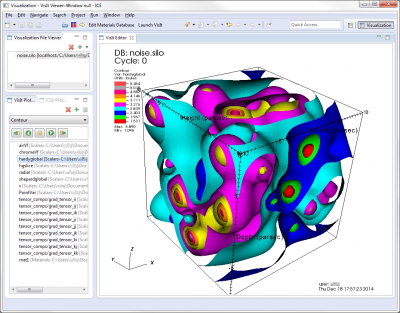
\includegraphics[width=\textwidth]{figures/ICE_VisIt.png}
\caption{A contour plot shown in the ICE VisIt Editor. }
\end{figure}

\begin{figure}[htbp]
\centering
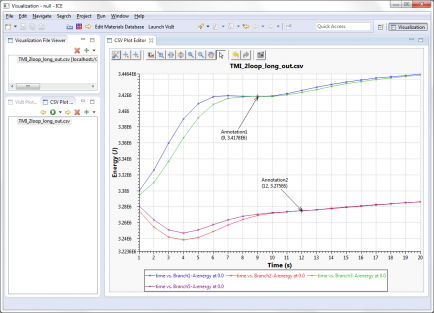
\includegraphics[width=\textwidth]{figures/ICE_CSVPlotter.png}
\caption{The ICE CSV Plot Editor showing MOOSE PostProcessor data.}
\end{figure}
\newpage
%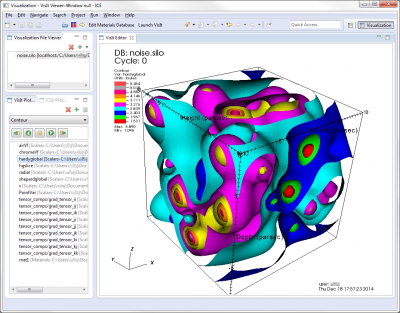
\includegraphics{figures/ICE_VisIt.png} 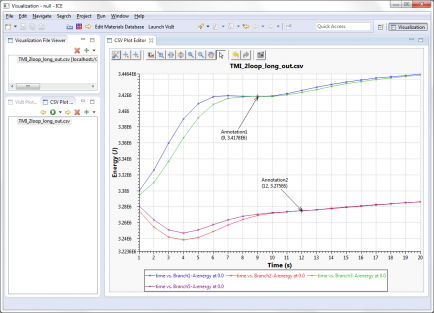
\includegraphics{figures/ICE_CSVPlotter.png}

\section{Installation and
Configuration}\label{installation-and-configuration}

\subsection{Prerequisites}\label{prerequisites}

To use the \emph{VisIt Tools}, ICE requires the installation of
\href{https://wci.llnl.gov/simulation/computer-codes/visit/}{VisIt}
(minimum version 2.8.2) developed by Lawrence Livermore National
Laboratory, either locally or on a remote machine.

The \emph{CSV Plotting Tools} require no additonal software to be
installed.

\subsection{Visualization
Perspective}\label{visualization-perspective}

To use ICE's visualization tools, you first must switch to the
\emph{Visualization Perspective}. This perspective includes various UI
components necessary for visualization that are not exposed in the
default ICE perspective. To access the \emph{Visualization Perspective},
use the the main menu bar at the top of the window and navigate to:

\emph{Window} \textgreater{} \emph{Open Perspective} \textgreater{}
\emph{Other}...

Select \emph{Visualization} in the dialog that pops up and click
\emph{OK}. Alternatively, you can also access the same pop-up dialog by
clicking the \emph{Open Perspective} button in the main toolbar in the
upper right-hand corner of the ICE workbench.

\begin{figure}[htbp]
\centering
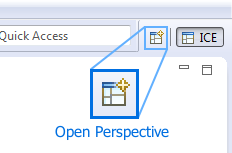
\includegraphics{figures/ICE_OpenPerspective.png}
\caption{The Open Perspective button for switching to another perspective, like in this case, the Visualization Perspective.}
\end{figure}

Once the \emph{Visualization Perspective} opens, you should notice the
workbench contains some new UI components. Make note of the following
panels, as we will be referring to them in the following sections.

\begin{figure}[htbp]
\centering
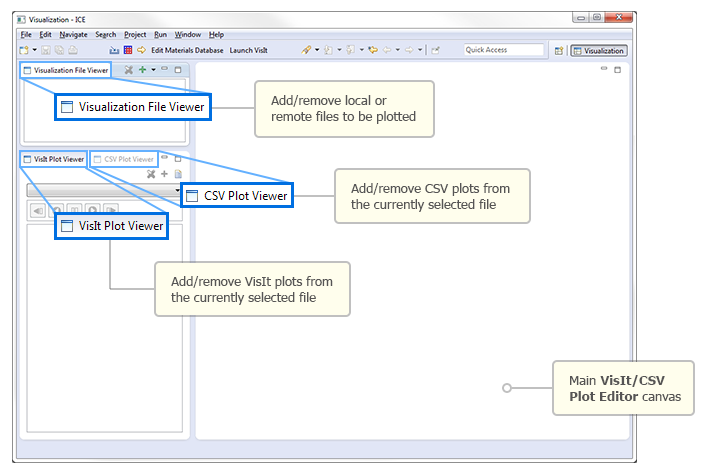
\includegraphics[width=\textwidth]{figures/ICE_VisualizationPerspective.png}
\caption{The ICE Visualization Perspective.}
\end{figure}

\section{Visualizing Output}\label{visualizing-output}

\subsection{VisIt}\label{visit}

\paragraph{Connecting to VisIt}\label{connecting-to-visit}

Once you switch to the \emph{Visualization Perspective}, the first step
necessary is to connect to your VisIt installation through ICE. To do
this, click on the \emph{Launch VisIt} button located in the ICE toolbar
near the top.

\begin{figure}[htbp]
\centering
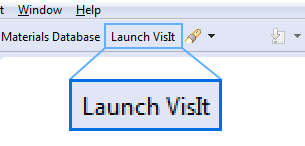
\includegraphics{figures/ICE_VisItLaunchButton.png}
\caption{The Launch VisIt button in the ICE toolbar.}
\end{figure}

A dialog will pop up offering you three options for connecting to VisIt:

\begin{figure}[htbp]
\centering
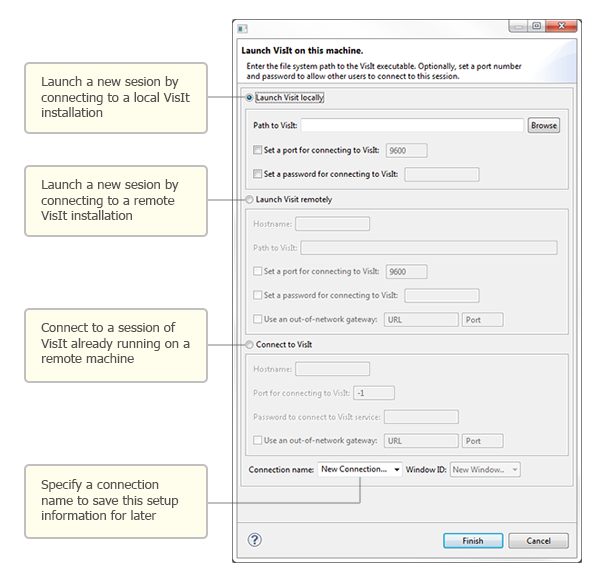
\includegraphics[width=\textwidth]{figures/ICE_VisItLaunchOptions.png}
\caption{The VisIt connection wizard in ICE.}
\end{figure}

\begin{enumerate}
\itemsep1pt\parskip0pt\parsep0pt
\item
  \textbf{Launch VisIt locally}\\If you installed VisIt on your local
  machine, use the \emph{Browse} button to direct ICE to your local
  installation directory. Using this method of connecting will launch a
  new VisIt session. Optionally, you can also set a port number (default
  9600) and-\/-if you want to share your VisIt session with another
  user-\/-a password.
\item
  \textbf{Launch VisIt remotely}\\If you installed VisIt on a remote
  machine, specify the hostname and full path to the VisIt installation
  directory. Using this method of connecting will launch a new VisIt
  session. Optionally, you can specify a port number (default 9600)
  and-\/-if you want to share your VisIt session with another user-\/-a
  password. If you need or want to use an external gateway or proxy to
  access the remote VisIt installation, you may specify its URL and port
  number as well.
\item
  \textbf{Connect to VisIt}\\If you would like to connect to session of
  VisIt already running somewhere else, specify the hostname, port
  number, and password set on the VisIt session; you will need to obtain
  this information from the person who initially launched the VisIt
  session. If you need or want to use an external gateway or proxy to
  access the remote VisIt installation, you may specify its URL and port
  number as well.
\end{enumerate}

Regardless of which method you choose to connect to VisIt, enter a
\emph{Connection name} at the bottom of the pop-up dialog. This will
allow you to re-use this connection information in the future.

If you are connecting to an existing session, specify a \emph{Window ID}
between 1 and 16. Which \emph{Window ID} you use depends on how you
would like to connect to VisIt. If multiple users connect using the same
\emph{Window ID}, they will all see and be able to interact with the
same VisIt view. However, if you would like multiple users to each have
their own unique session each with its own controls, assign a unique
\emph{Window ID} to each user. The VisIt installation can support up to
16 unique window IDs at a time.

Once you are done, click the \emph{Finish} button at the bottom, and ICE
should begin connecting to VisIt.

\paragraph{Adding/Removing Files}\label{addingremoving-files}

To open a file, find the green + icon in the \emph{Visualization File
Viewer}. Clicking directly on the green + icon will prompt a local
file browser to pop up. However, if your file is located on a remote
machine, or if you would like to add a file set, click on the drop-down
button next to the green + icon.

\begin{figure}[htbp]
\centering
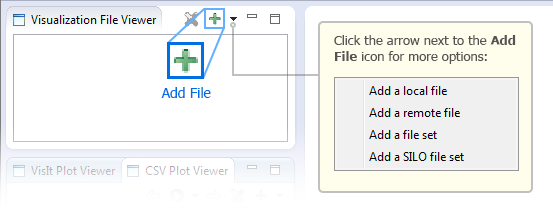
\includegraphics[width=\textwidth]{figures/ICE_VisItAddFileButton.png}
\caption{To add a new file to view in VisIt, click the green Add File button in the Visualization File View toolbar.}
\end{figure}

This will offer you four ways to open file(s):

\begin{itemize}
\itemsep1pt\parskip0pt\parsep0pt
\item
  Open a local file
\item
  Open a remote file
\item
  Open a local file set
\item
  Open a local SILO set
\end{itemize}

Once you have selected your file(s), they should appear in the
\emph{Visualization File Viewer}.

Lastly, if you would like to remove a file from the \emph{Visualization
File Viewer} list, select it, and click the red ``X'' button.

\paragraph{Adding/Removing Plots}\label{addingremoving-plots}

To begin adding plots, select your file in the \emph{Visualization File
Viewer} and click the green + icon in the \emph{VisIt Plot Viewer}.

\begin{figure}[htbp]
\centering
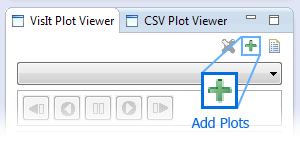
\includegraphics{figures/ICE_VisItAddPlotButton.png}
\caption{To add a new plot, click the Add Plots button in the VisIt Plot Viewer toolbar. }
\end{figure}

If there is any plottable data in your file, a dialog will pop up with a
list of options to choose from. This can include mesh plots, scalar
plots, vector plots, material block plots, and so forth. If there are
multiple plots of each type available, you can select them all by
checking off the entire category, or expand it to check off only
selected plots.

\begin{figure}[htbp]
\centering
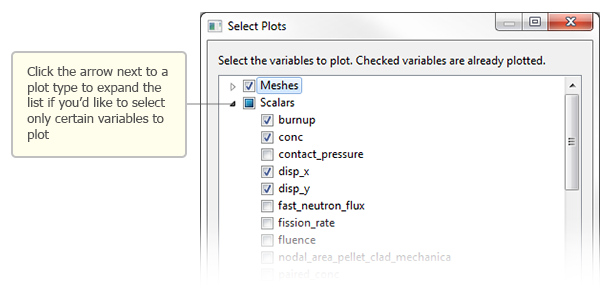
\includegraphics[width=\textwidth]{figures/ICE_VisItPlotSelection.png}
\caption{ICE prompts you with a list of available plots to select from. }
\end{figure}

When you are done selecting your plot(s), click \emph{OK}. The selected
plots should be added to the list in the \emph{VisIt Plot Viewer}.

Lastly, if you would like to remove a plot from the \emph{VisIt Plot
Viewer} list, select it and click the red ``X'' button.

\paragraph{Rendering Plots}\label{rendering-plots}

To render a plot, \emph{double} click it in the \emph{VisIt Plot
Viewer}, and it will appear in the main \emph{VisIt Editor}.

The \emph{VisIt Plot Viewer} contains a drop-down menu with a list of
plotting styles available for the currently selected plot. Depending on
your selected plot, this can include mesh, pseudo-color, contour,
volume, and so forth. Use this drop-down menu to select the plotting
style you prefer, and the \emph{VisIt Editor} will update in real time.

\begin{figure}[htbp]
\centering
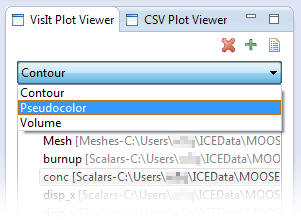
\includegraphics{figures/ICE_VisItPlotStyleMenu.png}
\caption{You can select the plot type in the VisIt Plot Viewer drop-down menu.}
\end{figure}

The \emph{VisIt Editor} is also interactive in that you can move your
plot around by clicking and dragging the canvas or zoom by using the
mouse wheel. This may not necessarily be useful for 2D plots but enables
a fully rotatable look at 3D plots as in the example below.

\begin{figure}[htbp]
\centering
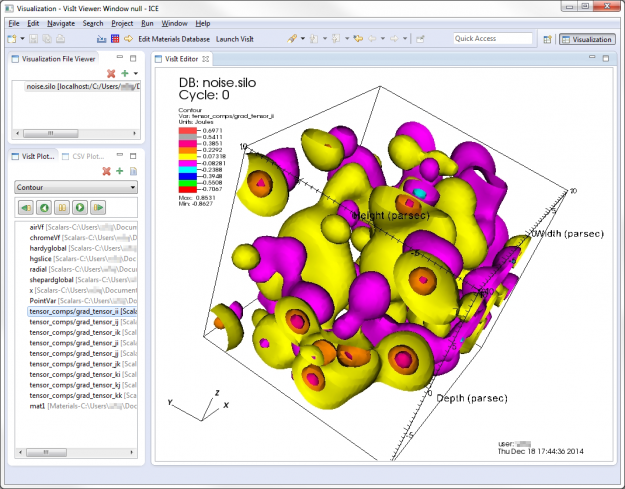
\includegraphics[width=\textwidth]{figures/ICE_VisIt3DNoise.png}
\caption{A view of a sample plot in the Visit Editor.}
\end{figure}

Lastly, if there is any time series data associated to your plot, you
can manually walk through the time steps, or play them continuously as a
short video, using the playback buttons located in the \emph{VisIt Plot
Viewer}.

\begin{figure}[htbp]
\centering
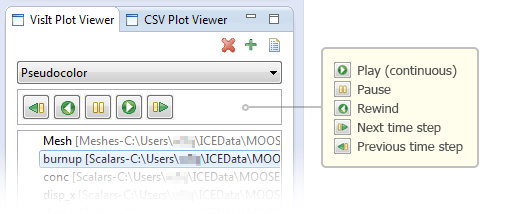
\includegraphics[scale=.6]{figures/ICE_VisItPlaybackButtons.png}
\caption{For time-series data, you can play through all time steps with the playback buttons in the Visit Plot Viewer. }
\end{figure}

\paragraph{Executing Python Commands}\label{executing-python-commands}

While many of VisIt's features are already accessible in ICE, work to
enable a more robust feature set is on-going. In the meantime, features
not yet integrated into ICE can still be accessed via Python commands by
clicking the Python script button located in the \emph{VisIt Plot
Viewer}.

\begin{figure}[htbp]
\centering
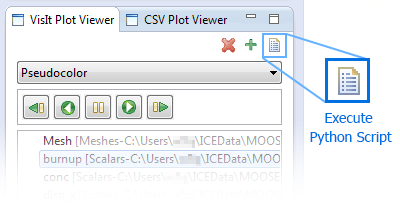
\includegraphics[scale=.6]{figures/ICE_VisItPythonScriptButton.png}
\caption{You can manipulate a VisIt plot with Python commands using the Execute Python Script button in the VisIt Plot Viewer.}
\end{figure}

Writing Python scripts for VisIt is beyond the scope of this tutorial.
However, you are welcome to refer to the
\href{https://wci.llnl.gov/simulation/computer-codes/visit/manuals}{VisIt
Python Interface Manual} provided by the VisIt development team at
Lawrence Livermore National Laboratory.

\subsubsection{CSV Plot Viewer}\label{csv-plot-viewer}

ICE includes, out of the box, basic CSV data plotting utilities for fast
and easy x/y graph visualizations. This section describes how to open
your CSV data using the \emph{CSV Plot Viewer} in the
\emph{\hyperref[Visualizationux5fPerspective]{Visualization
Perspective}}.

\paragraph{Adding/Removing Files}\label{addingremoving-files-1}

To open a file, find the green + icon in the \emph{Visualization File
Viewer}. Clicking directly on the green + icon will prompt a local
file browser to pop up. You can also access this option by clicking on
the drop-down button next to the green + icon.

\begin{figure}[htbp]
\centering
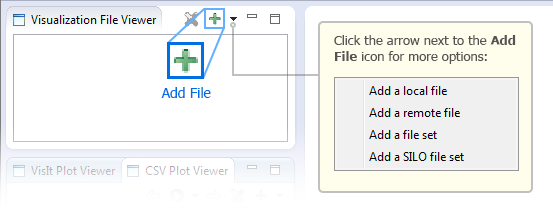
\includegraphics[width=\textwidth]{figures/ICE_VisItAddFileButton.png}
\caption{The VisIt Add File sub-menu.}
\end{figure}

This will offer you four ways to open file(s):

\begin{itemize}
\itemsep1pt\parskip0pt\parsep0pt
\item
  Open a local file
\item
  Open a remote file
\item
  Open a local file set
\item
  Open a local SILO set
\end{itemize}

Once you have selected your file(s), they should appear in the
\emph{Visualization File Viewer}.

Lastly, if you would like to remove a file from the \emph{Visualization
File Viewer} list, select it, and click the red ``X'' button.

\paragraph{Adding/Removing Plots}\label{addingremoving-plots-1}

\subparagraph{Adding Plots}\label{adding-plots}

To begin adding plots, select your file in the \emph{Visualization File
Viewer} and click the green + icon in the \emph{CSV Plot Viewer}.

\begin{figure}[htbp]
\centering
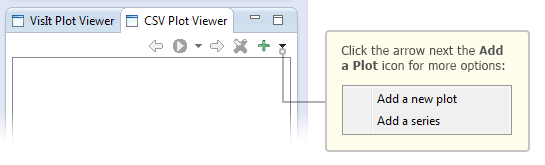
\includegraphics[width=\textwidth]{figures/ICE_CSVAddPlotButton.png}
\caption{The CSV Add Plot button.}
\end{figure}

\subparagraph{Selecting Initial Plot
Data}\label{selecting-initial-plot-data}

If the data in your CSV file is properly formatted, then a dialog will
appear. This dialog gives you a list of variables from your data file.

\begin{figure}[htbp]
\centering
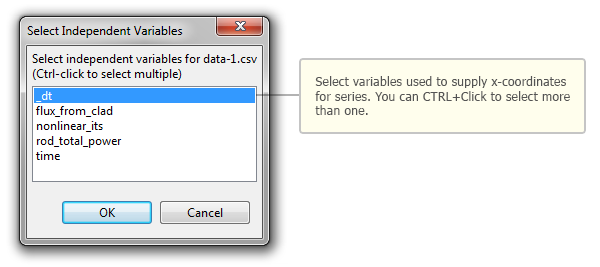
\includegraphics[width=\textwidth]{figures/ICE_CSVAddPlotDialog-XAxisVariables.png}
\caption{The CSV Add Plot independent variables dialog. }
\end{figure}

In this first dialog, you select independent variables from your CSV
file. Independent variables are those whose values determine the
x-coordinates of plotted series. You can select multiple data as
independent variables by holding the \emph{CTRL} key while clicking
values in the dialog's list. When you are finished selecting independent
variables from the list, click \emph{OK} or press \emph{Enter}.

A second dialog allowing you to select the plot type will appear. The
default plot type is \emph{Line}, which when used means the
xy-coordinates of added series will be connected by a line. The plot
type selected from this dialog will be used for all series generated
from this sequence of dialogs.

\begin{figure}[htbp]
\centering
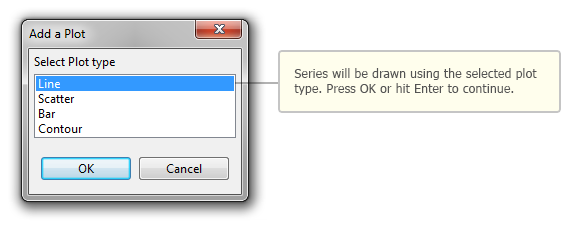
\includegraphics[scale=.6]{figures/ICE_CSVAddPlotDialog-PlotTypes.png}
\caption{The CSV plot type dialog.}
\end{figure}

Once you have chosen your desired plot type, click \emph{OK} or press
\emph{Enter}.

A third dialog allowing you to select the features that will actually be
plotted will appear.

\begin{figure}[htbp]
\centering
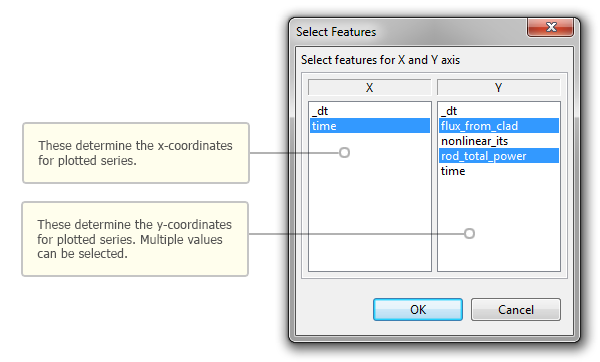
\includegraphics[width=\textwidth]{figures/ICE_CSVAddPlotDialog-Features.png}
\caption{ The CSV Plot features dialog.  }
\end{figure}

The list on the left includes the \emph{independent variables} selected
in one of the previous dialogs. You must select at least one of these
independent variables, as they provide the \emph{x}-coordinates of
series generated from the dialog.

The list on the right includes all \emph{features} available in the
file. You must select at least one of these features, as they provide
the \emph{y}-coordinates of series generated from the dialog.

You can also select multiple variables from either list by holding the
\emph{CTRL} key while clicking variables, although you should note that
every combination of selected independent (x) and feature (y) variables
will be plotted.

Once you have selected your desired x- and y-axis variables, click
\emph{OK} or press \emph{Enter}. A new plot will be added to the list in
the \emph{CSV Plot Viewer}. To open this plot, simply click it, and it
will open in a new \emph{CSV Plot Editor}.

\begin{figure}[htbp]
\centering
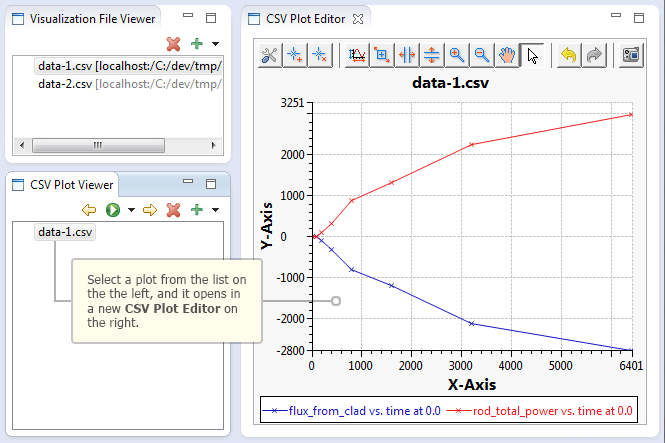
\includegraphics[width=\textwidth]{figures/ICE_CSVPlotEditor.png}
\caption{The ICE CSV Plot Editor. }
\end{figure}

\subparagraph{Showing/Moving Plots}\label{showingmoving-plots}

To re-open an existing plot, click its item in the \emph{CSV Plot
Viewer}, which is usually located on the left. The associated \emph{CSV
Plot Editor} in the main workbench space will be brought to the top or
activated. You can also click on the associated \emph{CSV Plot Editor}'s
tab to open it, or you can click and drag its tab to move it to another
spot in your workbench.

\begin{figure}[htbp]
\centering
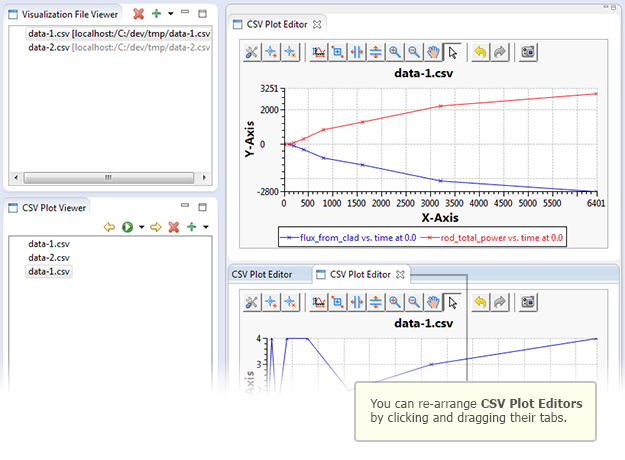
\includegraphics[width=\textwidth]{figures/ICE_CSVPlotEditor-Moved.png}
\caption{You can move multiple plots around through mouse-click and drag.}
\end{figure}

\subparagraph{Removing Plots}\label{removing-plots}

Lastly, if you would like to remove a plot from the \emph{CSV Plot
Viewer} list, select it and click the red ``X'' button. To permanently
remove it from view, you will also need to close the \emph{CSV Plot
Editor} in the main workbench space.

\paragraph{Adding Series to a Plot}\label{adding-series-to-a-plot}

To add more series to an existing \emph{CSV Plot Editor}, you must first
select the desired plot in the \emph{CSV Plot Viewer}. Locate the green
+ button in the \emph{CSV Plot Viewer} and click on the drop-down
button next to it. Select \emph{Add a series}.

You will then be prompted with the same sequence of dialogs as in the
section on \hyperref[Selectingux5fInitialux5fPlotux5fData]{Selecting
Initial Plot Data}.

When you have finished selecting plot data as described in that section,
the new data will be added to your selected plot as new series.

\paragraph{Plot Toolbar}\label{plot-toolbar}

The plotting widget used by ICE's \emph{CSV Plot Editor} includes a
toolbar with helpful utilities for navigating your plotted data or
customizing the plot's appearance. You can hover the mouse cursor over
each button to view a tool tip describing what the button does.

Clicking the first button will open a dialog that allows you to
customize the appearance of the plot or individual series on the plot,
including titles, scales, grids, colors, and fonts. The last button
allows you to save the current appearance of the plot to a \texttt{.png}
image file. Feel free to try out the different utilities available in
this toolbar.
